% @file           thesis.tex
% @brief          graduation thesis of Shibaura Institute of Technology
% @author         Kataoka Nagi al18036[at]shibaura-it.ac.jp
% @date           2021-12-21 15:19:48
% $Version:       1.0
% @par            History
%                 add
% Copyright (c) 2021 Kataoka Nagi

\documentclass[12pt,a4j]{jreport}
\setcounter{secnumdepth}{5}
\usepackage[dvipdfmx]{graphicx}
\usepackage{amsmath,amssymb}
\usepackage{comment}
\usepackage{graphicx}
\usepackage{here}
\usepackage{bm}
\usepackage{url}

\renewcommand{\baselinestretch}{1.5}

\renewcommand{\bibname}{参考文献}





\begin{document}


%%%%%%%%%%%%%%%%%%%%%%%%%%%%%%%%%%%%%
% 表紙
%%%%%%%%%%%%%%%%%%%%%%%%%%%%%%%%%%%%%
\begin{titlepage}

\begin{center}

    \vspace*{2cm}
    \Large 2021 年度 芝浦工業大学 工学部 情報工学科\\

    \vspace*{1.0cm}
    \Huge 卒 \qquad 業 \qquad 論 \qquad 文\\
    \vspace*{2.5cm}

    \Large 記事トピックのクラスタを用いた\\多言語ニュース推薦手法の提案
    
    \vspace{4cm}
    \begin{tabular}{ll}
        \vspace*{2mm}
        学籍番号 & \qquad $\mathbf{AL18036}$ \\
        \vspace*{2mm}
        氏\phantom{  }名 & \qquad 片岡 \quad 凪   \\
        \vspace*{2mm}
        指導教員           & \qquad 木村 \quad 昌臣
    \end{tabular}
\end{center}
\end{titlepage}



% \begin{abstract}
% このファイルは,情報工学科卒業論文の推奨テンプレートである.概要書とは異なり,卒業論文本体のテンプレートはあくまで推奨であるので,このテンプレートを下にして文字サイズや行間などを修正したものを利用しても良く,またこのテンプレートを使わなくても良い.

% この部分の研究概要では,研究背景,解決したい問題,研究目的,提案手法,評価方法,評価の結果について簡潔に書く.
% 概要の有無は任意.
% \end{abstract}


{\makeatletter
\let\ps@jpl@in\ps@empty
\makeatother
\pagestyle{empty}
\tableofcontents
\clearpage}

\setcounter{page}{1} 
\pagestyle{plain}

%%%%%%%%%%%%%%%%%%%%%%%%%%%%%%%%%%%%%%%%%%%%%%%%%%%%%%%%%%%%%
% 書式 
%%%%%%%%%%%%%%%%%%%%%%%%%%%%%%%%%%%%%%%%%%%%%%%%%%%%%%%%%%%%%
% 図の参照『図\ref{fig_nn}に3層のニューラルネットワークを示す』
% \begin{figure}[ht]
% 	\centering
% 	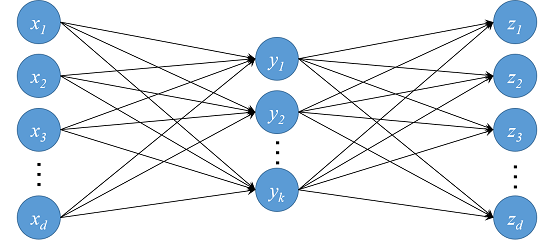
\includegraphics[keepaspectratio, width=120mm]{img/sample.png}
% 	\caption{提案法に用いた3層のニューラルネットワーク.キャプションにはこの図の説明を書く.}
% 	\label{fig_nn}
% \end{figure}

% 表の参照『表\ref{table_a}に手法Aおよび手法Bの正答率を示す』
% \begin{table}[ht]
%   \caption{手法Aおよび手法Bの正解率と平均計算時間.}
%   \label{table_a}
%   \centering
%   \begin{tabular}{lcr}
%     \hline
%     手法   & 正解率[\%]  &  計算時間[ms]  \\
%     \hline \hline
%     手法A  & 92.3  & 512 \\
%     手法B  & 87.4  & 32  \\
%     \hline
%   \end{tabular}
% \end{table}

% 参考文献『井尻らは,X線CTとデジタルカメラを用いた3次元モデリング法を提案した\cite{Ijiri18}.』
% 参考文献リスト『著者1, 著者2,...,著者N. タイトル. 論文誌or学会名, 巻, 号, ページ, 発表年. 』
% Webページ『著者. ページタイトル. ページURL(2021年7月31日参照).』


%%%%%%%%%%%%%%%%%%%%%%%%%%%%%%%%%%%%%%%%%%%%%%%%%%%%%%%%%%%%%
% 序論 
%%%%%%%%%%%%%%%%%%%%%%%%%%%%%%%%%%%%%%%%%%%%%%%%%%%%%%%%%%%%%
\chapter{序論(この章タイトルは一例.各自内容に合わせてつけること)}

\section{背景}


\subsection{図表参照の例,}

%%%%%%%%%%%%%%%%%%%%%%%%%%%%%%%%%%%%%%%%%%%%%%%%%%%%%%%%%%%%%
% 序論 
%%%%%%%%%%%%%%%%%%%%%%%%%%%%%%%%%%%%%%%%%%%%%%%%%%%%%%%%%%%%%

\subsection{関連研究参照の例}

\section{Latexファイルのコンパイル方法}

\subsection{ローカルにLatex環境を構築する場合}

\subsection{Overleafを利用する場合}


\section{目的}



\section{本論文の構成}



%%%%%%%%%%%%%%%%%%%%%%%%%%%%%%%%%%%%%%%%%%%%%%%%%%%%%%%%%%%%%
%%%%%%%%%%%%%%%%%%%%%%%%%%%%%%%%%%%%%%%%%%%%%%%%%%%%%%%%%%%%%
\chapter{関連研究}

\section{グループ1}

\section{グループ2}




%%%%%%%%%%%%%%%%%%%%%%%%%%%%%%%%%%%%%%%%%%%%%%%%%%%%%%%%%%%%%
%%%%%%%%%%%%%%%%%%%%%%%%%%%%%%%%%%%%%%%%%%%%%%%%%%%%%%%%%%%%%
\chapter{提案手法}

\section{設計指針}

\section{システム構成}

\section{ユーザインタフェース}

\section{アルゴリズム}




%%%%%%%%%%%%%%%%%%%%%%%%%%%%%%%%%%%%%%%%%%%%%%%%%%%%%%%%%%%%%
%%%%%%%%%%%%%%%%%%%%%%%%%%%%%%%%%%%%%%%%%%%%%%%%%%%%%%%%%%%%%
\chapter{評価実験}


\section{仮説}
% 評価実験を設計するにあたり以下3件の仮説を立てる.
% \begin{itemize}
%   \item 仮説1) .
%   \item 仮説2) 
%   \item 仮説3) 
% \end{itemize}
% この3件の仮設は,それぞれ以下の考察に基づき設定されている.
% 仮説1は...


\section{実験手順}




%%%%%%%%%%%%%%%%%%%%%%%%%%%%%%%%%%%%%%%%%%%%%%%%%%%%%%%%%%%%%
%%%%%%%%%%%%%%%%%%%%%%%%%%%%%%%%%%%%%%%%%%%%%%%%%%%%%%%%%%%%%
\chapter{結果と考察}


\section{実験1について}


\section{実験2について}





%%%%%%%%%%%%%%%%%%%%%%%%%%%%%%%%%%%%%%%%%%%%%%%%%%%%%%%%%%%%%
%%%%%%%%%%%%%%%%%%%%%%%%%%%%%%%%%%%%%%%%%%%%%%%%%%%%%%%%%%%%%
\chapter{まとめと展望}





\chapter*{謝辞}
\addcontentsline{toc}{chapter}{謝辞}

\bibliographystyle{junsrt}
\bibliography{ref.bib}


\end{document}
